% UC Davis poster built from the Gemini theme
% (https://github.com/anishathalye/gemini) and inspired by
% Rylan Schaeffer's Stanford template
% (https://github.com/RylanSchaeffer/Stanford-LaTeX-Poster-Template).
%
% COMPILE WITH XeLaTeX (Overleaf: Menu > Settings > Compiler > XeLaTeX).
% The Gemini theme uses fontspec, which requires XeLaTeX or LuaLaTeX.
\documentclass[final]{beamer}

% ====================
% Packages
% ====================

\usepackage[T1]{fontenc}
\usepackage{lmodern}
\usepackage[size=custom,width=120,height=72,scale=1.0]{beamerposter}
\usetheme{gemini}
\usecolortheme{ucdavis}
\usepackage{graphicx}
\usepackage{booktabs}
\usepackage{tikz}
\usepackage{pgfplots}
\pgfplotsset{compat=1.17}

% ====================
% Lengths
% ====================

% Three-column layout: 4 separators + 3 cols = paperwidth
\newlength{\sepwidth}
\newlength{\colwidth}
\setlength{\sepwidth}{0.025\paperwidth}
\setlength{\colwidth}{0.3\paperwidth}

\newcommand{\separatorcolumn}{\begin{column}{\sepwidth}\end{column}}

% ====================
% Title / authors
% ====================

\title{Risk Estimation of Preeclampsia}

\author{Ahmed Khan \and Lawrencedel Legaspi \and Selena Phu}

\institute[shortinst]{Department of Electrical and Computer Engineering}

% ====================
% Footer
% ====================

\footercontent{
  \href{https://github.com/AhmedKhan-GH/repnet}{github.com/AhmedKhan-GH/repnet} \hfill
  UC Davis Senior Design Showcase 2026 \hfill \phantom{}}

% ====================
% Logos: UC Davis ECE logo (left), RUbiNet project logo (right)
% ====================

\logoleft{
\includegraphics[height=9cm]{logo.png}}
\logoright{
\includegraphics[height=5.5cm]{ece_header_white_text.png}}

% ====================
% Custom Headline Template to Include Poster Number
% ====================
\makeatletter
\setbeamertemplate{headline}
{
  \begin{beamercolorbox}{headline}
    \begin{columns}
      % Left Logo Column
      \begin{column}{\maxlogowidth}
        \vskip5ex
        \ifdefined\insertlogoleft
        \vspace*{\fill}
        \hspace{10ex}
        \raggedright
        \insertlogoleft
        \vspace*{\fill}
        \else\fi
      \end{column}
      
      % Center Title/Author/Institute Column
      \begin{column}{\dimexpr\paperwidth-\maxlogowidth-\maxlogowidth}
        \usebeamerfont{headline}
        \vskip3ex
        \centering
        {\usebeamerfont{headline title}\usebeamercolor[fg]{headline title}\inserttitle\\[0.5ex]}
        {\usebeamerfont{headline author}\usebeamercolor[fg]{headline author}\insertauthor\\[1ex]}
        {\usebeamerfont{headline institute}\usebeamercolor[fg]{headline institute}\insertinstitute\\[1ex]}
      \end{column}
      
      % Right Logo & Poster Number Column
      \begin{column}{\maxlogowidth}
        \vskip3ex
        % Fixed alignment: zero-width box keeps it close to the right edge with clear safety padding
        \hfill\makebox[0pt][r]{\usebeamerfont{headline title}\textbf{\Huge 117}\hspace{2ex}}\par
        \vskip2ex
        \ifdefined\insertlogoright
        \vspace*{\fill}
        \raggedleft
        \insertlogoright
        \hspace{10ex}
        \vspace*{\fill}
        \else\fi
      \end{column}
    \end{columns}
    \vspace{5ex}
    \ifbeamercolorempty[bg]{headline rule}{}{
      \begin{beamercolorbox}[wd=\paperwidth,colsep=0.25ex]{headline rule}\end{beamercolorbox}
    }
  \end{beamercolorbox}
}
\makeatother

% ====================
% Body
% ====================

\begin{document}

\begin{frame}[t]
\begin{columns}[t]
\separatorcolumn

% =========================================================
% Column 1: Context & Strategy
% =========================================================
\begin{column}{\colwidth}

  \begin{block}{Introduction}
    Preeclampsia is a hypertensive disorder that may occur after 20 weeks of pregnancy. It can cause liver damage, low platelet count, preterm birth, etc. If left unaddressed, the disorder can rapidly worsen to Eclampsia, meaning it will affect brain function, putting the mother at risk of comas or seizures. As there is no immediate treatment for Preeclampsia outside of childbirth, it is imperative to find a way to predict a mother's risk of the disorder so steps can be taken to prevent it. To do this, we use different methods of machine learning on 12-Lead ECGs to accurately predict risk.
  \end{block}

  \begin{block}{Future Work}
    \begin{itemize}
      \item \textbf{Lead Reduction:} Instead of using 12 leads of ECG data, a reduction in amount of leads may be enough in detecting preeclampsia.
      \item \textbf{Feature Importance Across Models:} Feature importance selection in this project were results of a Random Forest model, though models such as CatBoost or LightGBM may find other features removed useful. This has the possibility of improving performance metrics at the cost of more features.
      \item \textbf{MUSE derived features:} During NeuroKit validation in the earlier stages of the project, instead of deriving novel features from the raw ECGs, it was possible to derive comparable features using only MUSE-reported data. Current models used MUSE + extracted NeuroKit features, but what if derived MUSE features were used instead?
    \end{itemize}
  \end{block}

  \begin{block}{Acknowledgements}
    \textbf{Faculty Advisors:} Lihong Mo, MD, PhD, Assistant Professor, Obstetrics \& Gynecology; Chen-Nee Chuah, Professor, Electrical \& Computer Engineering

    \vskip0.5ex
    \textbf{Grad Alum/Student Mentors:} Hana Shaik and Arielle Yoo

    \vskip0.5ex
    \textbf{Institution:} UC Davis
  \end{block}

\end{column}

\separatorcolumn

% =========================================================
% Column 2: Convolutional Neural Networks
% =========================================================
\begin{column}{\colwidth}

  \begin{block}{CNN Models for ECG Feature Learning}
  \end{block}

\end{column}

\separatorcolumn

% =========================================================
% Column 3: Decision-Tree Information (Methods & Results)
% =========================================================
\begin{column}{\colwidth}

  \begin{block}{Decision-Tree Methods}
    UC Davis Health was able to provide an unbalanced dataset of ECGs with already reported features exported from a GE MUSE 12L system. This dataset contains 329 preeclamptic ECGs and 1830 normal ECGs for a split of 15.2\%/84.8\%.

    \begin{enumerate}
      \item Preprocess ECG data using NeuroKit2 to extract more features
      \item Add extracted NeuroKit2 features to the MUSE reported dataset
      \item Apply feature importance methods
      \begin{itemize}
        \item Pearson Correlation
        \item ANOVA
        \item Recursive Feature Elimination
      \end{itemize}
      \item Train decision-tree models
    \end{enumerate}

    Original feature importance and modeling was performed on a Random Forest model using 5-fold StratifiedGroupKFold and RandomUnderSampler. Eventually, testing of other decision-tree models and ensembles were performed to obtain better results.
  \end{block}

  \begin{block}{Decision-Tree Results}
    Unweighted Voting with SVM and LogisticRegression proved to be the best model when focusing on sensitivity/balanced accuracy. We look at these metrics to understand how well the model is correctly identifying preeclamptic ECGs and whether or not the model is genuinely distinguishing correctly between a normal or preeclamptic ECG.

    \begin{table}
      \centering
      \small
      \resizebox{\colwidth}{!}{%
      \begin{tabular}{l c c c c c c c}
        \toprule
        \textbf{Ensemble} & \textbf{AUROC} & \textbf{AUPRC} & \textbf{Specificity} & \textbf{Sensitivity} & \textbf{Balanced Accuracy} & \textbf{Precision} & \textbf{F1-Score} \\
        \midrule
        Unweighted Voting & 74.54 $\pm$ 4.16 & 41.81 $\pm$ 7.86 & 74.26 $\pm$ 3.95 & 59.32 $\pm$ 10.70 & 66.79 $\pm$ 3.60 & 29.25 $\pm$ 1.38 & 38.94 $\pm$ 2.99 \\
        Weighted Voting & 74.75 $\pm$ 4.48 & 42.26 $\pm$ 7.92 & 74.75 $\pm$ 4.48 & 60.23 $\pm$ 10.88 & 67.49 $\pm$ 3.45 & 30.05 $\pm$ 1.57 & 39.80 $\pm$ 2.76 \\
        Unweighted Voting + SVM, LR & 75.72 $\pm$ 3.94 & 41.58 $\pm$ 8.03 & 74.64 $\pm$ 4.70 & 62.35 $\pm$ 10.93 & 68.50 $\pm$ 3.22 & 30.72 $\pm$ 1.08 & 40.85 $\pm$ 2.24 \\
        Stacking & 74.77 $\pm$ 4.35 & 42.43 $\pm$ 7.59 & 74.37 $\pm$ 4.18 & 59.62 $\pm$ 10.80 & 67.00 $\pm$ 3.46 & 29.45 $\pm$ 1.20 & 39.17 $\pm$ 2.79 \\
        Bagging CatBoost & 74.81 $\pm$ 4.98 & 41.96 $\pm$ 8.86 & 74.70 $\pm$ 4.68 & 59.62 $\pm$ 15.19 & 67.16 $\pm$ 5.59 & 29.49 $\pm$ 2.51 & 39.10 $\pm$ 5.21 \\
        \bottomrule
      \end{tabular}%
      }
      \caption{Performance comparison of tree-based ensemble methods on the UCDH dataset.}
    \end{table}

    \vskip2ex
    To identify the most robust cardiological markers for preeclampsia and eliminate noisy variables, we evaluated our engineered feature space across multiple selection feature importances: Pearson Correlation, ANOVA, and RFE (scoring on balanced accuracy, rocauc, and average precision). 

    \begin{figure}
      \centering
      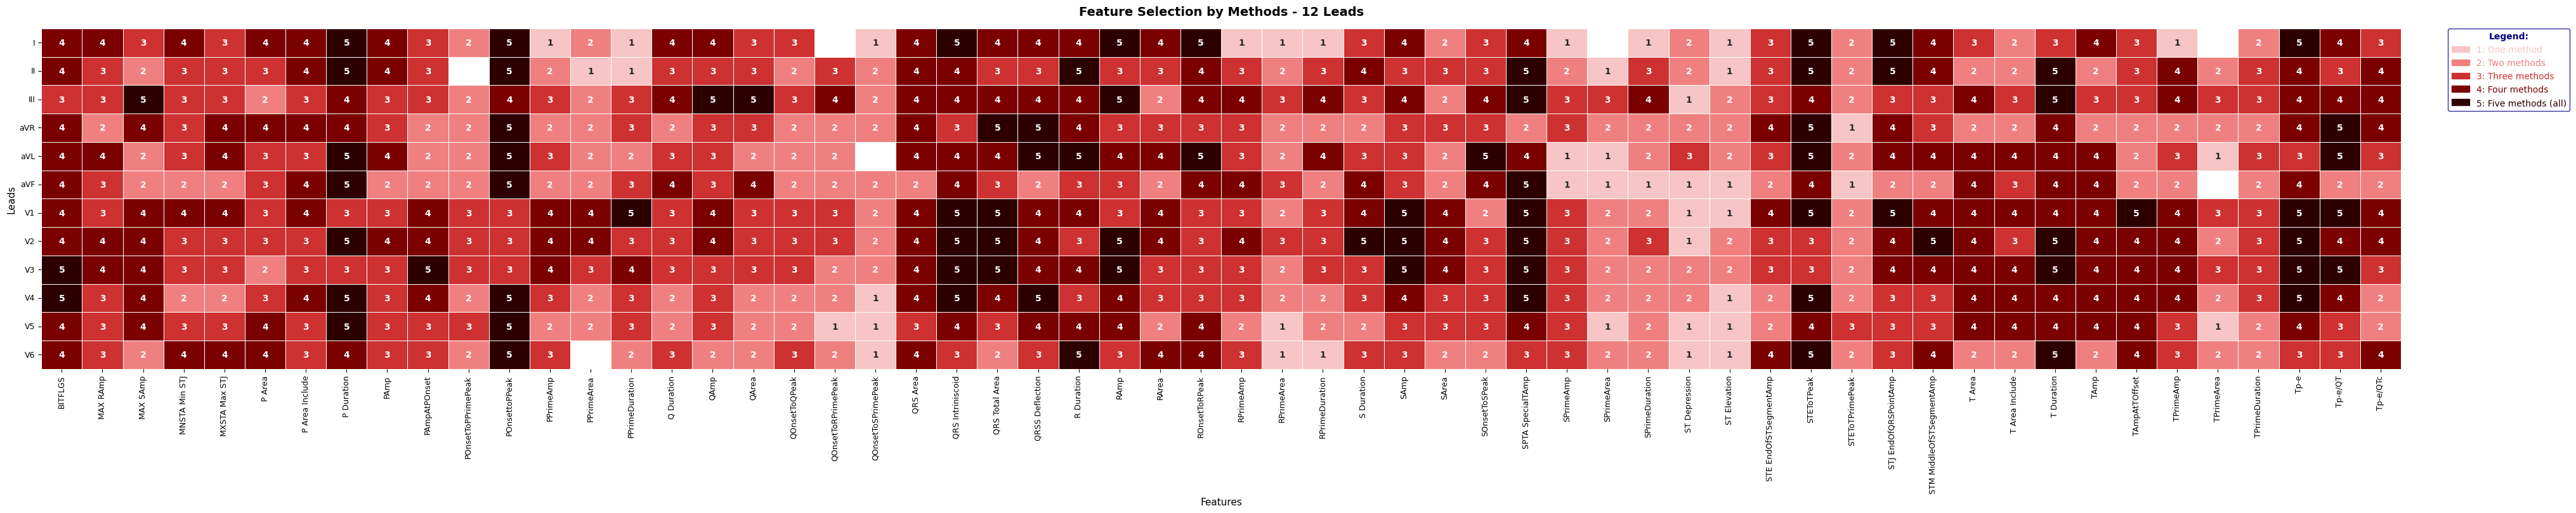
\includegraphics[width=0.98\colwidth]{Heatmap12leads.png}
      \caption{Feature Selection consensus heatmap across 12 ECG leads.}
    \end{figure}

    The horizontal distribution illustrates consensus across feature importances, where darker blocks reveal important features for the lead. Global features are not reported here.
  \end{block}

\end{column}

\separatorcolumn
\end{columns}
\end{frame}

\end{document}